% =====================================================================================
% Configuration generation (Task 1): the protocol that produced the pool of candidate structures.
% SOURCES: PaperData/plan-docs/Task1_configuration_generation_plan.md (v1.4+), the generators
% PaperData/code/sampleGen/{common.py,s1..s8,s5supercell}, PaperData/Task1_output/task1_summary.csv,
% PaperLatex/configurationGeneration.tex (earlier version of this text). Rewritten in full sentences 2026-10-15;
% small energies converted to atomic units (1 meV = 36.75 microHa; 0.05 eV/A = 9.7e-4 Ha/Bohr).
% =====================================================================================

\section{Configuration generation and sampling}
\label{sec:configgen}

The training data of the machine-learned force fields are built in three steps: configuration
generation, which is described here, down-sampling in descriptor space, and DFT labelling (main
text, \emph{Identifying structures for DFT labelling}). Configuration generation produces a
deliberately oversampled pool of \num{55928} structures of \CsSnI{}, \MASnI{} and \FASnI{}. The pool
has to span, with margin, every state that the production simulations visit: the $\alpha$, $\beta$
and $\gamma$ perovskite phases and the transitions between them, temperatures from the orthorhombic
phase to above the cubic transition, the lattice strains produced by thermal expansion, by the
spontaneous strain of each transition and by substrate clamping, and disordered orientations of the
molecular cations.

\subsection{Sampling model and molecular-dynamics engine}
\label{sec:configgen:engine}

\paragraph{Sampling model.} The structures are sampled with our in-house foundation model. For
sampling, the neighbour-list capacities in the header of the model file were enlarged from (76, 40)
to (120, 60) neighbours. These numbers size buffers only: energies, forces and stresses are bitwise
identical to those of the original file, but compressed low-temperature hybrid cells need more than
the original radial capacity. The model only proposes plausible structures. Every structure selected
for labelling is recomputed with DFT, so the errors of the sampling model affect where configuration
space is sampled but never the labels.

\paragraph{Rejected alternative.} We first tested a public general-purpose foundation
model\cite{Song2024NEP89} and rejected it. In \SI{50}{ps} constant-volume runs at the experimental
volume it collapsed the \CsSnI{} framework at \SIlist{300;500}{\kelvin} and the \MASnI{} and
\FASnI{} frameworks already at \SI{200}{\kelvin}, producing Sn--Sn distances of
\SI{2.7}{\angstrom} and mean Sn--I coordination numbers of 2.9 to 5.4.

\paragraph{Engine.} All sampling MD uses the batched GPU engine of UrsaMLFF (commit
\texttt{4f4f697e1}). It integrates the equations of motion in double precision and accumulates
forces in 64-bit fixed point, so that a run is bitwise reproducible for a given input and seed, and
it evaluates many independent systems concurrently on one GPU. Two engine defects found during this
work are fixed in that commit and are documented and tested in the engine repository. First,
trajectory frames written during constant-pressure runs carried the cell of the start of the run
segment. Second, in cells thinner than $2.5(r_\mathrm{c}+r_\mathrm{skin})$ the engine uses explicit
periodic-image atoms, and a system that outgrew the image region sized at start-up was integrated
with missing periodic images until the next output frame; atoms are now wrapped into the cell at
every regeneration of the images, and an overflowing system is stopped immediately. All data reported
here were generated after both fixes.

\paragraph{Qualification.} Before sampling we checked the model in three ways. First, along an
isotropic energy--volume scan the pressure obtained from the stress equals $-\mathrm{d}E/\mathrm{d}V$;
the zero-pressure pseudo-cubic lattice constants are \SI{6.29}{\angstrom} for \CsSnI{} and about
\SI{6.40}{\angstrom} and \SI{6.49}{\angstrom} for \MASnI{} and \FASnI{}, 1 to \SI{3}{\percent}
larger than experiment, as expected for a PBE-based model. Second, in constant-volume MD at the
experimental volume the Sn--I framework stays intact from \SIrange{200}{500}{\kelvin} for all three
compounds, with a mean Sn--I coordination of at least 5.9 and no Sn--Sn distance below
\SI{5}{\angstrom}; these runs were repeated with the corrected engine. Third, in flexible
constant-pressure MD at \SI{0}{\giga\pascal}, \CsSnI{} at \SI{500}{\kelvin} and both hybrids at
\SI{300}{\kelvin} expand without bound (pseudo-cubic lattice constants above \SI{7.2}{\angstrom}
for the hybrids) and their frameworks decompose (Sn--Sn distances of about \SI{2.7}{\angstrom}),
because the model lacks restoring forces on expansion of these compounds. At \SI{0.5}{\giga\pascal}
\MASnI{} still decomposes at \SI{400}{\kelvin}. We therefore apply a constant pressure correction of
$P^\ast=+\SI{1.0}{\giga\pascal}$ to every constant-pressure run. At this pressure the model reproduces
the experimental volume with every framework intact: the pseudo-cubic lattice constant is
\SI{6.200}{\angstrom} for \CsSnI{} at \SI{500}{\kelvin} (experiment \SI{6.206}{\angstrom}), and
\SI{6.310}{\angstrom} and \SI{6.381}{\angstrom} for \MASnI{} and \FASnI{} at \SI{400}{\kelvin}
(experiment \SI{6.240}{\angstrom} and \SI{6.316}{\angstrom} at room temperature). Stage S2 also
samples $P^\ast\pm\SI{0.2}{\giga\pascal}$, so that the pool is not tied to a single pressure.

\subsection{Seed structures}
\label{sec:configgen:seeds}

\paragraph{Cell family.} The barostat of the engine acts on axis-aligned orthorhombic cells, so all
constant-pressure sampling uses a single cell family, the $\sqrt{2}a\times\sqrt{2}a\times2a$
pseudo-cubic cell of four formula units with the doubled axis along $z$. This cell hosts the
$a^0a^0a^0$ ($Pm\bar{3}m$), $a^0a^0c^+$ ($P4/mbm$), $a^0a^0c^-$ ($I4/mcm$) and $a^-a^-c^+$ ($Pnma$)
tilt systems exactly orthogonally, so a heating or cooling run can cross
$\alpha\leftrightarrow\beta\leftrightarrow\gamma$ inside one cell. A pseudo-cubic
$2\times2\times2$ cell would not do, because it is monoclinic by \ang{0.33} for $Pnma$. The sampling
cells are $2\times2\times2$ repetitions for \CsSnI{} (160 atoms) and $2\times2\times1$ repetitions for
\MASnI{} and \FASnI{} (192 atoms), both below the limit of 200 atoms set for DFT labelling.

\paragraph{Glazer-tilt frameworks.} The three phases of each compound are built by rigid octahedral
rotations with the Glazer pattern of the phase\cite{Glazer1972} and then rescaled axis by axis to the
experimental lattice parameters of \CsSnI{},\cite{Chung2012JACS}
\MASnI{}\cite{Mitzi1995JSSC,stoumpos2013semiconducting} and \FASnI{}\cite{schueller2018crystal}
(Table~\ref{tab:seeds}). No verified lattice of the low-temperature orthorhombic phase of \MASnI{} is
available, so for that phase the $\beta$ lattice contracted by 0.3 to \SI{0.6}{\percent} is used. The
tilt angles of the seeds are only starting values and are re-equilibrated at temperature before any
frame is kept.

\paragraph{Molecular cations.} MA$^+$ and FA$^+$ are placed as rigid ideal cations with independent,
uniformly random orientations on every A site. The orientations are drawn after the supercell is
built, so that no period-two pattern is inherited, and placements with H$\cdots$I distances below
\SI{2.35}{\angstrom} or intermolecular H$\cdots$H distances below \SI{1.9}{\angstrom} are rejected.
Each hybrid phase is seeded with two independent orientation draws, and one polar-aligned \MASnI{}
seed with all C$\to$N vectors along $+z$ is added at low weight.

\paragraph{Materials Project seeds.} The Materials Project\cite{mp2013} contributes structures that
tilting an ideal perovskite cannot produce: the edge-sharing yellow $\delta$ phase of \CsSnI{}, the
DFT-relaxed $\gamma$ phase of \CsSnI{} with its A-site displacements and Sn off-centring,
cation-ordered \MASnI{} (antipolar $Pnma$ and polar) and \FASnI{} ($Amm2$) structures, and, at low
weight, the decomposition products Cs$_2$SnI$_6$, SnI$_2$ and CsI. Their Materials Project
identifiers are listed in the main text.

\paragraph{Substitution-derived seeds.} Nine further frameworks are derived from ABX$_3$ entries of
neighbouring chemistries, Pb analogues, bromides and chlorides, by transmutation to Sn and I.
Deduplication with a symmetry-tolerant structure matcher reduced 37 candidates to 14 distinct
frameworks, of which nine are used. Each is rescaled isotropically to the pseudo-cubic lattice
constant of the target compound, with the molecular cations moving as rigid units. Transmutation
transfers the topology (connectivity, tilt pattern and cation ordering) but not the geometry, and the
tilt amplitudes are reset by equilibration. These seeds add three further antipolar MA orderings, a
partially aligned MA ordering ($Cc$) and the $a^0a^0c^-$ tilt pattern for \CsSnI{}.

\paragraph{Non-diagonal supercells.} A diagonal supercell forces every tilt and cation-orientation
pattern to repeat every two pseudo-cubic units. We therefore also build the smallest supercells
beyond that period-two repeat, the non-diagonal supercells of a pseudo-cubic $2\times2\times2$
cell,\cite{LloydWilliams2015PRB} which at a comparable atom count hold more independent cation
orientations and tilt patterns. The framework inside is the same $\alpha$, $\beta$ or $\gamma$
perovskite, so these cells are a choice of periodicity, not a different phase. The supercell matrix
$Q=[[0,1,1],[1,0,1],[1,1,0]]$ gives 16 formula units (80 atoms for \CsSnI{}, 192 for the hybrids)
with a minimum width of about $2.3a_\mathrm{pc}$, against $2.0a_\mathrm{pc}$ for the diagonal
16-formula-unit hybrid cell; $Q=[[\bar1,1,1],[1,\bar1,1],[1,1,\bar1]]$ gives 32 formula units
(160 atoms, \CsSnI{} only) with a minimum width of about $2.8a_\mathrm{pc}$. Because these cells are
not orthogonal, they are sampled at constant volume.

\begin{table}[tb]
\caption{Glazer-tilt seed frameworks. Lattice parameters are those of the orthorhombic
$\sqrt{2}\times\sqrt{2}\times2$ setting (\si{\angstrom}), with the temperature at which they were
measured. Tilt angles are starting values only; they relax during equilibration. The Materials
Project IDs of the direct and substitution-derived seeds are listed in Table~\ref{tab:mp}.}
\label{tab:seeds}
\begin{tabular}{llllll}
\toprule
 & Phase & Glazer & Lattice (\si{\angstrom}) & $T$ (K) & Ref. \\
\midrule
\CsSnI{} & $\alpha$, $Pm\bar{3}m$ & $a^0a^0a^0$ & $a=6.206$ & $\approx500$ & \cite{Chung2012JACS} \\
 & $\beta$, $P4/mbm$ & $a^0a^0c^+$ & 8.712, 6.191 & $\approx380$ & \cite{Chung2012JACS} \\
 & $\gamma$, $Pnma$ & $a^-a^-c^+$ & 8.688, 8.643, 12.378 & 300 & \cite{Chung2012JACS} \\
\MASnI{} & $\alpha$ & $a^0a^0a^0$ & $a=6.240$ & 298 & \cite{Mitzi1995JSSC} \\
 & $\beta$, $I4cm$ & $a^0a^0c^-$ & 8.758, 12.429 & 200 & \cite{stoumpos2013semiconducting} \\
 & $\gamma$ & $a^-a^-c^+$ & $\beta\times(0.997,0.994,0.997)$ & -- & -- \\
\FASnI{} & $\alpha$, $Pm\bar{3}m$ & $a^0a^0a^0$ & $a=6.316$ & 298 & \cite{schueller2018crystal} \\
 & $\beta$, $P4/mbm$ & $a^0a^0c^+$ & 8.862, 6.249 & 175 & \cite{schueller2018crystal} \\
 & $\gamma$, $Pnma$ & $a^-a^-c^+$ & 8.817, 8.858, 12.416 & 100 & \cite{schueller2018crystal} \\
\bottomrule
\end{tabular}
\end{table}

% moved from the main text (2026-10-29, methods condensed)
\begin{table}[htbp]
  \centering
  \caption{Materials Project\cite{mp2013} structures used as starting points for the sampling MD,
    with their space groups. Substitution sources were transmuted to the composition in the last
    column and rescaled to its pseudo-cubic lattice constant. The structures were retrieved through
    the Materials Project API on 28 September 2026.}
  \label{tab:mp}
  \begin{tabular}{llll}
    \toprule
    ID & structure & space group & used as \\
    \midrule
    \multicolumn{4}{l}{\emph{used directly}} \\
    mp-568570 & \CsSnI{}, $\gamma$ phase & $Pnma$ & \CsSnI{} \\
    mp-27381 & \CsSnI{}, yellow (edge-sharing) phase & $Pnma$ & \CsSnI{} \\
    mp-1094059 & \MASnI{}, antipolar MA order & $Pnma$ & \MASnI{} \\
    mp-995238 & \MASnI{}, polar MA order & $P1$ & \MASnI{} \\
    mp-1102654 & \FASnI{} & $Amm2$ & \FASnI{} \\
    mp-27636 & Cs$_2$SnI$_6$ & $Fm\bar{3}m$ & reference \\
    mp-27194 & SnI$_2$ & $C2/m$ & reference \\
    mp-614603 & CsI & $Fm\bar{3}m$ & reference \\
    \midrule
    \multicolumn{4}{l}{\emph{substitution sources}} \\
    mp-1014168 & CsPbBr$_3$ & $I4/mcm$ & \CsSnI{} \\
    mp-1120725 & CsPbBr$_3$ & $Amm2$ & \CsSnI{} \\
    mp-27394 & CsSnCl$_3$ & $P2_1/c$ & \CsSnI{} \\
    mp-995203 & MAPbI$_3$ & $Pnma$ & \MASnI{} \\
    mp-995214 & MAPbI$_3$ & $Pnma$ & \MASnI{} \\
    mp-1194604 & MAPbI$_3$ & $Pnma$ & \MASnI{} \\
    mp-995227 & MAPbI$_3$ & $Cc$ & \MASnI{} \\
    mp-2646983 & FASnBr$_3$ & $Cm$ & \FASnI{} \\
    mp-977014 & FAPbI$_3$ & $Pmm2$ & \FASnI{} \\
    \bottomrule
  \end{tabular}
\end{table}

\subsection{Sampling stages}
\label{sec:configgen:stages}

Seven complementary sampling stages (S1 to S7), one stage of larger cells (S5$'$) and one
dipole-targeted stage (S8) target different parts of configuration space; Table~\ref{tab:si-stages}
summarises them.

\paragraph{S1, volume--shape grid (constant volume).} Every phase seed is run at 11 affine cell shapes,
each at three temperatures spanning the stability range of the phase and its neighbours
(Table~\ref{tab:tgrid}). The shapes are isotropic scalings by 0.970, 0.985, 1.000, 1.015 and 1.030,
biaxial in-plane strains of $\pm1$ and $\pm\SI{2}{\percent}$ (the substrate-clamping mode) and
tetragonal strains of the $c$ axis of $\pm\SI{2}{\percent}$ (the Poisson response). Holding the cell
fixed at known strains supplies the stress labels from which the force field learns the elastic
response, on which the clamping study depends, and anchors the sampling at the experimental volume
independently of the equation of state of the sampling model.

\paragraph{S2, heating and cooling ramps (constant pressure).} Flexible constant-pressure MD at
$P^\ast$ is ramped linearly over \SI{150}{\pico\second}, from 100 to \SI{600}{\kelvin} for \CsSnI{}
(\SI{3.3}{\kelvin\per\pico\second}) and from 50 to \SI{450}{\kelvin} for the hybrids
(\SI{2.7}{\kelvin\per\pico\second}). The ramps start from each phase and run in both directions, the
hybrids are cooled from two orientation draws, and heating ramps at $P^\ast\pm\SI{0.2}{\giga\pascal}$
are added. These ramps generate transition-crossing configurations, both hysteresis branches and the
spontaneous transition strain, which constant-volume runs suppress. They are several hundred times
faster than the ramps used to locate the transition temperatures (main text, \emph{Phase
identification}) and serve for sampling only.

\paragraph{S3, near-$T_\mathrm{c}$ boundary conditions (constant pressure).} The $\beta$ and $\alpha$
seeds are run for \SI{100}{\pico\second} at three temperatures bracketing each transition,
\SIlist{340;380;430}{\kelvin} for \CsSnI{}, \SIlist{250;275;300}{\kelvin} for \MASnI{} and
\SIlist{200;240;280}{\kelvin} for \FASnI{}, under the two mechanical conditions of the production
study: an in-plane tension of \SI{50}{\mega\pascal}, with pressures of $(P^\ast-0.05, P^\ast-0.05,
P^\ast)$~GPa, and a rigid in-plane clamp, realised by an effectively infinite in-plane barostat
modulus with the normal free at $P^\ast$. The response of tilts and cation orientations to clamping
is largest near $T_\mathrm{c}$, where a force field trained only on free cells could not be trusted.

\paragraph{S4, robustness.} Constant-volume runs of \SI{100}{\pico\second} beyond the production range,
at \SI{700}{\kelvin} for \CsSnI{} and \SI{500}{\kelvin} for the hybrids, supply configurations that
keep the force field from failing when production MD fluctuates beyond the training range. The
polar-aligned \MASnI{} seed, run at \SIlist{150;300}{\kelvin}, tests the stability of aligned MA
order.

\paragraph{S5 and S5$'$, non-diagonal and larger cells.} The non-diagonal supercells are run at
constant volume at the upper two temperatures of their phase for \SI{100}{\pico\second} each, which
samples tilt and orientation correlations free of period-two constraints. Stage S5$'$ adds
$3\times3\times2$ \CsSnI{} cells (360 atoms), a 54-formula-unit non-diagonal supercell of a pseudo-cubic
$3\times3\times3$ cell (270 atoms, $\alpha$ phase only) and $3\times3\times1$ hybrid cells (432 atoms),
each run at one temperature per phase for \SI{100}{\pico\second}, at constant volume and, for the
orthorhombic cells, also at constant pressure. These cells hold correlated tilt and orientation
domains of about three pseudo-cubic units and are labelled directly.

\paragraph{S6 and S7, Materials Project and substitution-derived seeds.} These seeds are run at
constant volume (non-orthogonal cells) or at constant pressure at $P^\ast$ (orthorhombic cells), at
temperatures appropriate to each structure, with heating ramps for the ordered $\gamma$-type seeds.
They add phases, cation orderings and decomposition products that S1 to S5 cannot reach.

\paragraph{S8, dipole-targeted cation order (constant volume).} Seeds with prescribed molecular-dipole
arrangements were added after the orientation analysis described below showed that S1 to S7 contain
no polar cells. For \MASnI{} and \FASnI{} in the $\alpha$ and $\gamma$ frameworks (192 atoms), six
arrangements are built: fully polar arrangements ($|\langle\mathbf{d}\rangle|\approx0.97$) along a
pseudo-cubic $\langle100\rangle$, $\langle110\rangle$ or $\langle111\rangle$ direction, partially
polar arrangements ($|\langle\mathbf{d}\rangle|=0.60\pm0.03$) along $\langle100\rangle$ or
$\langle111\rangle$ drawn from a von Mises--Fisher distribution, and an antipolar arrangement with
dipoles alternating between layers. Only the rotation of each cation about its dipole axis is random.
Because the sampling model relaxes polar order within picoseconds above \SI{100}{\kelvin}, no
equilibration is discarded: after a fixed-cell relaxation, \SI{8}{\pico\second} of constant-volume MD
at \SIlist{50;150}{\kelvin} ($\gamma$) or \SIlist{150;300}{\kelvin} ($\alpha$) are sampled every
\SI{0.1}{\pico\second}. The runs thus cover the relaxation from the prescribed order to disorder and
every net polarisation in between; at \SI{50}{\kelvin} the polar order largely survives
($|\langle\mathbf{d}\rangle|\approx0.7$ after \SI{8}{\pico\second}), while at 150 to
\SI{300}{\kelvin} it decays to 0.2 to 0.3.

\begin{table}[tb]
\caption{S1 temperatures (K) per phase seed. Each seed is run at 11 cell shapes at each
temperature.}
\label{tab:tgrid}
\begin{tabular}{lccc}
\toprule
 & $\gamma$ & $\beta$ & $\alpha$ \\
\midrule
\CsSnI{} & 150, 300, 400 & 300, 400, 450 & 400, 500, 600 \\
\MASnI{} & 50, 100, 150  & 150, 250, 300 & 250, 350, 450 \\
\FASnI{} & 50, 100, 150  & 150, 200, 250 & 250, 350, 450 \\
\bottomrule
\end{tabular}
\end{table}

\subsection{Integration, thermostat, barostat and sampling frequency}
\label{sec:configgen:md}

\paragraph{Starting sequence.} Every run starts with a fixed-cell FIRE\cite{Bitzek2006PRL} relaxation
to a maximum force of \SI{9.7e-4}{\hartree\per\bohr} (at most 1000 steps), after which velocities are
drawn at the starting temperature and \SI{5}{\pico\second} of constant-volume MD with stochastic
velocity rescaling\cite{Bussi2007JCP} ($\tau_T=\SI{100}{\femto\second}$) precede the production
segment. Frames from these steps are discarded, except in the S2 ramps, which start from the
equilibrated state.

\paragraph{Time step.} The time step is \SI{1.0}{\femto\second} for \CsSnI{} and
\SI{0.5}{\femto\second} for the hybrids, because of the N--H and C--H stretches. We checked both
choices in \SI{5}{\pico\second} constant-energy runs from equilibrated states. For \CsSnI{} at
\SI{500}{\kelvin} the total energy is conserved to better than \SI{0.04}{\micro\hartree} per atom up
to a time step of \SI{2}{\femto\second}, with no measurable drift. For \MASnI{} at \SI{350}{\kelvin}
the energy fluctuation grows from 0.22 to \SI{0.92}{\micro\hartree} per atom between time steps of
0.25 and \SI{0.5}{\femto\second}, a factor of 3.8 close to the $\Delta t^2$ scaling of a stable
integration, and the drift at \SI{0.5}{\femto\second} is \SI{0.55}{\micro\hartree} per atom and
picosecond. At \SI{1}{\femto\second} the fluctuation grows a further 6.5-fold, to
\SI{5.9}{\micro\hartree} per atom, and the drift eighteen-fold, to \SI{9.9}{\micro\hartree} per atom and
picosecond, so that time step is too long for the hybrids.

\paragraph{Barostat.} Constant pressure uses stochastic cell rescaling\cite{Bernetti2020JCP} with
$\tau_P=\SI{1}{\pico\second}$, acting on each axis, with barostat moduli of 16, 14 and
\SI{12}{\giga\pascal} for \CsSnI{}, \MASnI{} and \FASnI{}. The moduli of the three axes differ in their
third decimal, because with equal pressures and equal moduli the engine performs shape-preserving
isotropic scaling, which would suppress the spontaneous transition strain.

\paragraph{Run length.} Production segments last \SI{100}{\pico\second} and the S2 ramps
\SI{150}{\pico\second}. At 250 to \SI{450}{\kelvin} the reorientation of MA$^+$ and FA$^+$ takes a few
picoseconds, so a segment spans tens of reorientation times. At 50 to \SI{150}{\kelvin} the
orientations are essentially frozen on this time scale, and the diversity there comes from the
independent orientation draws and the Materials Project orderings rather than from run length.
Octahedral tilt fluctuations decorrelate on the picosecond scale.

\paragraph{Sampling frequency and frame budget.} Stages S1 to S7 are budgeted at $5\times10^4$ frames
for the subsequent down-sampling, and the dipole-targeted stage S8 (\num{3936} frames) is added on top.
The budget is split between the compounds in proportion to their planned labelling budgets
(70:87:87 for \CsSnI{}:\MASnI{}:\FASnI{}), giving about \numlist{1.5e4;1.75e4;1.75e4} frames. At a
fixed segment length of \SI{100}{\pico\second} this sets the sampling interval to \SI{1}{\pico\second}
for \CsSnI{} (every \num{1000} steps), \SI{0.8}{\pico\second} for the hybrids (every \num{1600} steps)
and \SI{3.2}{\pico\second} for the large S5$'$ hybrid cells, which contain more independent local
environments per frame. Consecutive frames remain correlated on these intervals by design: the pool
is oversampled so that the down-sampling can select decorrelated, diverse frames. Each frame stores
the positions, the cell and the energy, forces and stress of the sampling model, which are used only
for descriptors and diagnostics.

\paragraph{Throughput and reproducibility.} All jobs share one run seed (2026), so the engine evaluates
jobs with identical protocols as a single batch of independent systems; batch members are always
distinct structures or temperatures, so their trajectories differ. The remaining protocol groups are
divided into shards that run concurrently on one GPU under the CUDA Multi-Process Service, which gives
a 2.7-fold speed-up for 192-atom systems; the trajectories are bitwise identical to those of sequential
execution. The S1 to S7 campaign of 449 jobs ran as 12 concurrent shards on a single NVIDIA A100 in
\SI{13}{\minute}: the 156 jobs of \CsSnI{} and its reference compounds in four shards, finished after
\SI{8}{\minute}, and the 293 hybrid jobs in eight shards, finished after \SI{13}{\minute}. All hybrid
jobs and 154 of the 156 \CsSnI{} jobs completed; the two exceptions are constant-volume runs of
Cs$_2$SnI$_6$ at \SIlist{300;500}{\kelvin}, which the temperature guard of the engine stopped, because
that compound lies outside the training domain of the sampling model. S8 was added afterwards as a
separate campaign of 48 jobs in three shards (\SI{10}{\second}), so the S1 to S7 inputs are unchanged by
it. The whole pool is regenerated bit for bit from the deposited job files and seed structures.

\begin{table}[tb]
\caption{Sampling stages. Ensembles, run lengths and frame counts after quality control and the
PAW-overlap cut. S6 also contributes 215 frames of the reference compounds Cs$_2$SnI$_6$, SnI$_2$ and
CsI, included in the total.}
\label{tab:si-stages}
\resizebox{\linewidth}{!}{%
\begin{tabular}{llllrrr}
\toprule
Stage & Ensemble & Seeds & Length & \CsSnI{} & \MASnI{} & \FASnI{} \\
\midrule
S1 & $NVT$, 11 shapes $\times$ 3 $T$ & Glazer $\alpha,\beta,\gamma$ & \SI{100}{\pico\second} & \num{9817} & \num{12298} & \num{12277} \\
S2 & $NPT$ ramps at $P^\ast$ ($\pm0.2$~GPa) & Glazer & \SI{150}{\pico\second} & \num{1248} & \num{2140} & \num{2144} \\
S3 & $NPT$, $-50$~MPa / clamp, near $T_\mathrm{c}$ & $\beta,\alpha$ & \SI{100}{\pico\second} & \num{1200} & \num{1500} & \num{1500} \\
S4 & $NVT$ hot; polar MA & $\alpha$ & \SI{100}{\pico\second} & \num{100} & \num{1051} & \num{245} \\
S5 & $NVT$, non-diagonal & Glazer & \SI{100}{\pico\second} & \num{1200} & \num{750} & \num{750} \\
S5$'$ & $NVT$ + $NPT$, 270--432 atoms & Glazer & \SI{100}{\pico\second} & \num{200} & \num{186} & \num{186} \\
S6 & $NVT$/$NPT$ & Materials Project & \SI{100}{\pico\second} & \num{310} & \num{875} & \num{250} \\
S7 & $NVT$/$NPT$ & substitution & \SI{100}{\pico\second} & \num{300} & \num{1000} & \num{250} \\
S8 & $NVT$, from $t=0$ & dipole-targeted & \SI{8}{\pico\second} & -- & \num{1968} & \num{1968} \\
\midrule
Total & & & & \num{14375} & \num{21768} & \num{19570} \\
\bottomrule
\end{tabular}}
\end{table}

\subsection{Quality control and PAW-overlap filter}
\label{sec:configgen:qc}

\paragraph{Integrity checks.} Every frame is checked for framework and molecular integrity. A frame is
rejected if its mean Sn--I coordination (within \SI{3.8}{\angstrom}) is below 5.5, if any Sn--Sn
distance is \SI{4.5}{\angstrom} or less, if any pair of Cs, Sn or I atoms is closer than
\SI{2.5}{\angstrom}, if a C--N bond is broken (one N per C for MA and two for FA within
\SI{1.7}{\angstrom}), if an H atom is detached, or if an H$\cdots$I distance is below
\SI{2.0}{\angstrom}. Frames failing these checks are not used as ordinary training data; the first
three per run are retained separately as candidate labels at the onset of failure, where the sampling
model is least reliable. In the pool, 1045 frames failed these checks.

\paragraph{PAW-overlap cut.} Because the labels are computed with the projector augmented-wave
method,\cite{Blochl1994PAW} we also cut on the overlap of the augmentation spheres. For each atom pair
we use the radii of the JTH datasets\cite{Jollet2014CPC} and the overlap measure of our DFT code,
\begin{equation}
  O_{ij} = \frac{r_i + r_j - d_{ij}}{r_i + r_j},
\end{equation}
where $r_i$ is the PAW radius of atom $i$ and $d_{ij}$ the pair distance, and remove frames with
$\max_{ij}O_{ij} \geq \SI{30}{\percent}$. In the hybrid frames the largest overlap is set by the C--H
bonds, with a median of \SI{20.6}{\percent}, a 99.9th percentile of \SI{25.5}{\percent} and a maximum
of \SI{27.96}{\percent}; \CsSnI{} frames have no overlap. Because the integrity checks already remove
the compressed configurations, the cut removes no frame from this pool and is kept as a safeguard for
later generations. The released pool therefore contains \num{55928} frames with or without the cut,
and the 70 failure-onset frames are provided separately.

\subsection{Down-sampling and labelled set}
\label{sec:configgen:down}
% moved from the main text (2026-10-29, methods condensed)
\paragraph{Down-sampling.}
Each atom of every pool structure was described by Gaussian multipole (GMP) descriptors\cite{Lei2019GMP, Lei2022GMP} (orders 0 to 5, ten Gaussian widths from 0.2 to \SI{2.0}{\angstrom}, scaled to the
unit interval). Environments closer than a cutoff distance in this space were treated as
equivalent, which leaves 3816 distinct environments. A greedy set cover, weighted by cell volume
as a proxy for the DFT cost, then selected the cheapest set of structures that together contain
all of them; the cutoff was set so that the cover holds 400 to 500 structures, and it selected
403. One further structure was added from each sampling stratum (a combination of stage,
compound, phase and cell deformation) that the cover had missed, the one farthest in descriptor
space from the structures already chosen (116 structures). A second round added 207 structures
of at most 200 atoms: 70 configurations from the onset of failures of the sampling model and
137 random structures, at most two per trajectory. Of these 726 structures, 718 were labelled
(main text, section \emph{Electronic structure}): 320 of \MASnI{}, 247 of \FASnI{}, 136 of \CsSnI{} and 15
of reference compounds, with 36 to 432 atoms. After the exclusion of one duplicate and two
Cs$_2$SnI$_6$ structures with unphysical Cs--I contacts, the PBEsol set used for training contains
715 structures. The \rSCAN{} set excludes the same three structures and ten \CsSnI{} cells whose
\rSCAN{} energies were affected by a numerical error in the meta-GGA implementation, since
corrected; it contains 705 structures.

\subsection{Active-learning labels}
\label{sec:configgen:al}
{\changedcolor
The PBEsol labels were extended in three rounds of active learning by 212 structures (main text,
Table~\ref{tab:labels}): cells of 192 atoms cut around the defect events of the hybrid MD, with their surroundings
re-equilibrated and the defect core fixed, images in which one N--H or C--H bond is stretched to between 1.03 and
\SI{1.6}{\angstrom}, and 27 frames of earlier out-of-distribution MD. The \rSCAN{} labels were computed for 185 of these
structures and for 20 of the out-of-distribution frames. A further 120 \rSCAN{} structures address the remaining
failures of the \rSCAN{} MD: scans of the Cs--Sn distance of a Cs ion entering a neighbouring cage (22 cells of 60
atoms), frames of \CsSnI{} (60 atoms), \MASnI{} and \FASnI{} (96 atoms) from MD at the highest temperatures (51), and
scans of short C--I and H--I contacts in \FASnI{} (31) and of C--I and N--I contacts in \MASnI{} (16), in cells of 96
atoms. Three \FASnI{} scan points whose largest force exceeds \SI{0.4}{\hartree\per\bohr} are not used, which leaves 117.
}

\subsection{Molecular-cation orientation and dipole statistics}
\label{sec:configgen:dipoles}

Because the response of the molecular cations to strain is central to this work, we analysed the
orientations of all \num{668848} MA$^+$ and FA$^+$ cations in the \num{41338} hybrid frames of the pool.
The dipole axis of MA$^+$ is the unit vector from C to N, and that of FA$^+$ the unit vector from the
midpoint of the two N atoms to C, which lies along the C--H bond and the molecular dipole. Orientations
are expressed in the pseudo-cubic frame of each frame, found as the rotation that best aligns the
Sn--Sn nearest-neighbour vectors with the Cartesian axes, so that they are comparable across cell
shapes, including the non-diagonal supercells.

\paragraph{Single-cation orientations.} Figure~\ref{fig:dipole_sphere} shows the orientation density
relative to an isotropic distribution. Above \SI{150}{\kelvin} both cations sample the sphere almost
uniformly: \SI{99.7}{\percent} of equal-area bins of the cubic fundamental zone are visited with at
least \SI{10}{\percent} of the isotropic density. At and below \SI{150}{\kelvin} the distributions
become anisotropic, as expected for orientationally ordered phases: MA$^+$ avoids the
$\langle111\rangle$ directions (coverage \SI{84}{\percent} in S1 to S7 and \SI{86}{\percent} with S8),
and FA$^+$ prefers directions near $\langle110\rangle$ (\SI{95.5}{\percent} and \SI{97.5}{\percent}).

\paragraph{Collective order.} In stages S1 to S7 the net polarisation $|\langle\mathbf{d}\rangle|$ of a
frame, averaged over its cations, follows the distribution of randomly oriented dipoles at every
temperature and never exceeds 0.64. Polar configurations are absent even though polar seeds were
included, because under the sampling model the fully polar \MASnI{} seed
($|\langle\mathbf{d}\rangle|=0.97$) depolarises to 0.45 within \SI{2}{\pico\second} at
\SI{150}{\kelvin}, inside the discarded equilibration. This finding motivated stage S8. With S8 the
pool contains 654 frames with $|\langle\mathbf{d}\rangle|>0.6$ and 145 with
$|\langle\mathbf{d}\rangle|>0.8$, up to 0.98, spread over all intermediate values
(Figure~\ref{fig:dipole_polar}). Nearest-neighbour pairs of cations favour antiparallel alignment at
low temperature and are nearly uncorrelated above \SI{150}{\kelvin} (Figure~\ref{fig:dipole_pairs}).

\begin{figure}[tb]
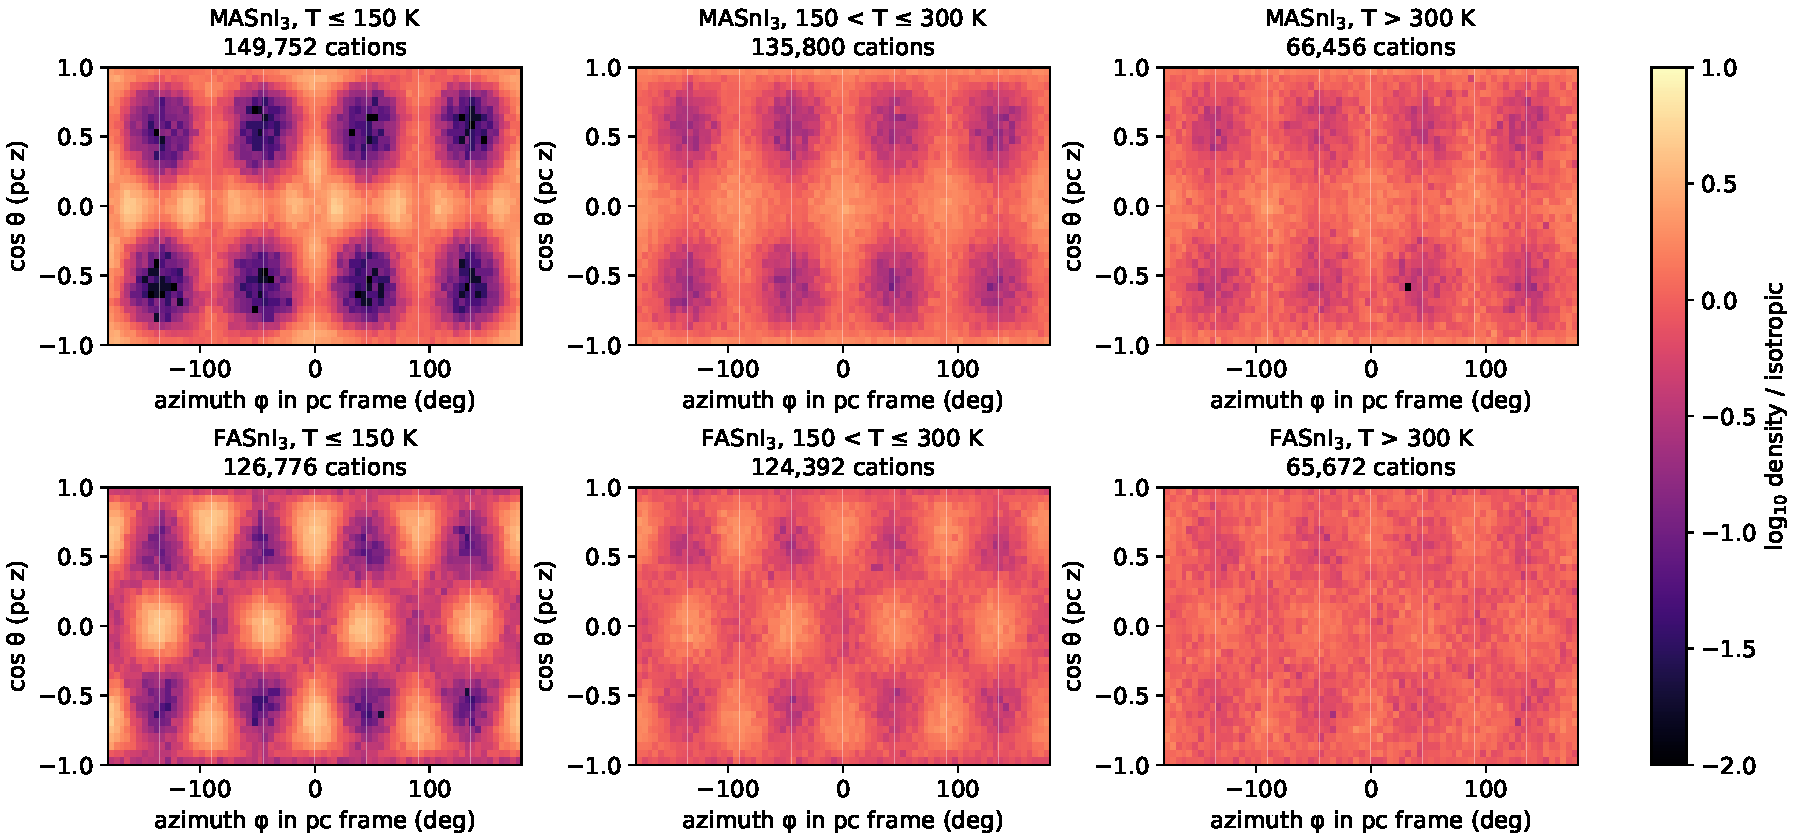
\includegraphics[width=\textwidth]{fig_dipole_sphere.pdf}
\caption{Orientation density of the molecular dipole axis (MA$^+$: C$\to$N; FA$^+$: N--N midpoint
$\to$C) in the pseudo-cubic frame, relative to an isotropic distribution (logarithmic colour scale),
for three temperature bands. Horizontal axis: azimuth; vertical axis: cosine of the polar angle, so
equal areas are equal solid angles.}
\label{fig:dipole_sphere}
\end{figure}

\begin{figure}[tb]
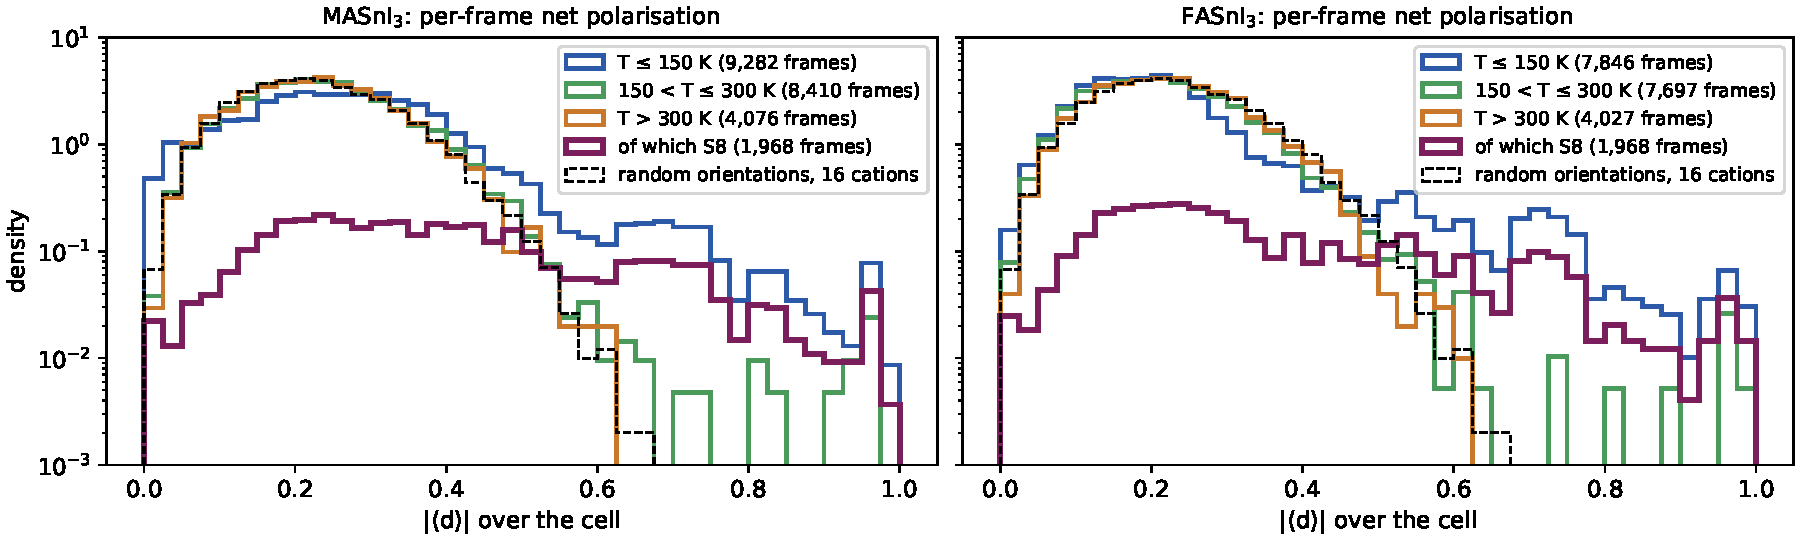
\includegraphics[width=\textwidth]{fig_dipole_polar.pdf}
\caption{Per-frame net polarisation $|\langle\mathbf{d}\rangle|$ of the molecular cations, for three
temperature bands (all stages), with the contribution of the dipole-targeted stage S8 (thick line)
and randomly oriented dipoles in a 16-cation cell (dashed). Logarithmic density scale.}
\label{fig:dipole_polar}
\end{figure}

\begin{figure}[tb]
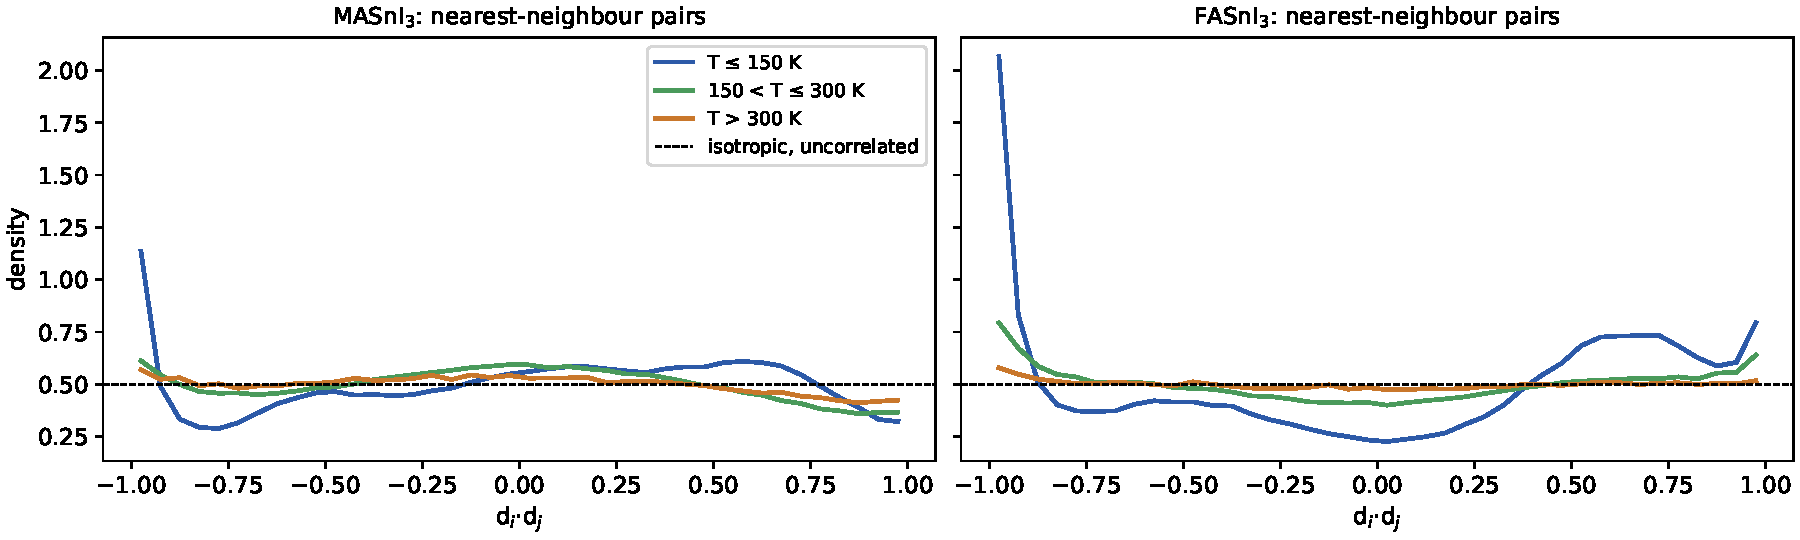
\includegraphics[width=\textwidth]{fig_dipole_pairs.pdf}
\caption{Distribution of the scalar product $\mathbf{d}_i\cdot\mathbf{d}_j$ of the dipole axes of
nearest-neighbour cation pairs in the pool, for \MASnI{} (left) and \FASnI{} (right) and three
temperature bands. The dashed line is the uniform density of isotropic, uncorrelated pairs. At and
below \SI{150}{\kelvin} antiparallel pairs ($\mathbf{d}_i\cdot\mathbf{d}_j\approx-1$) are enriched;
above it the distribution is close to uniform.}
\label{fig:dipole_pairs}
\end{figure}
